\section{Appendix D: Code Examples}
\label{sec:codeappendix}

\subsection{Ageing Error Estimation}
\hypertarget{AgeingError}{}
%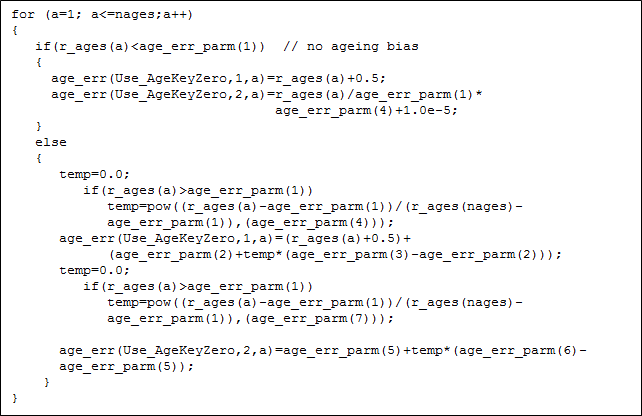
\includegraphics{age_error2}
%The 7 parameters are:

%\begin{itemize}
%	\item age at which the estimated pattern begins (just linear below this age).  This is “start age”
%	\item bias at start age (as additive offset from unbiased age’)
%	\item bias at maxage (as additive offset from unbiased age’)
%	\item power fxn coefficient for interpolating between those 2 values (value of 0.0 produces linear interpolation in the bias)
%	\item stdev at age
%	\item stdev at max age
%	\item power fxn coefficient for interpolating between those 2 values
%\end{itemize}

\scriptsize
\begin{verbatim}
 /*  SS_Label_FUNCTION 45 get_age_age */
 FUNCTION void get_age_age(const int Keynum, const int AgeKey_StartAge, const int AgeKey_Linear1, const int AgeKey_Linear2)
 {
 //  FUTURE: calculate adjustment to oldest age based on continued ageing of old fish
 age_age(Keynum).initialize();
 dvariable age;
 dvar_vector age_err_parm(1,7);
 dvariable temp;
 
 if(Keynum==Use_AgeKeyZero)
 {
 //  SS_Label_45.1 set age_err_parm to mgp_adj, so can be time-varying according to MGparm options
 for (a=1;a<=7;a++)
 {age_err_parm(a)=mgp_adj(AgeKeyParm-1+a);}
 age_err(Use_AgeKeyZero,1)(0,AgeKey_StartAge)=r_ages(0,AgeKey_StartAge)+0.5;
 age_err(Use_AgeKeyZero,2)(0,AgeKey_StartAge)=age_err_parm(5)*(r_ages(0,AgeKey_StartAge)+0.5)/
 (age_err_parm(1)+0.5);
 //  SS_Label_45.3 calc ageing bias
 if(AgeKey_Linear1==0)
 {
 age_err(Use_AgeKeyZero,1)(AgeKey_StartAge,nages)=0.5 + r_ages(AgeKey_StartAge,nages) + 
 age_err_parm(2)+(age_err_parm(3)-age_err_parm(2))*(1.0-mfexp(-age_err_parm(4)*
 (r_ages(AgeKey_StartAge,nages)-age_err_parm(1)))) / (1.0-mfexp(-age_err_parm(4)*
 (r_ages(nages)-age_err_parm(1))));
 }
 else
 {
 age_err(Use_AgeKeyZero,1)(AgeKey_StartAge,nages)=0.5 + r_ages(AgeKey_StartAge,nages) + 
 age_err_parm(2)+(age_err_parm(3)-age_err_parm(2))*
 (r_ages(AgeKey_StartAge,nages)-age_err_parm(1))/(r_ages(nages)-age_err_parm(1));
 }
 //  SS_Label_45.4 calc ageing variance
 if(AgeKey_Linear2==0)
 {
 age_err(Use_AgeKeyZero,2)(AgeKey_StartAge,nages)=age_err_parm(5)+(age_err_parm(6)-age_err_parm(5))*
 (1.0-mfexp(-age_err_parm(7)*(r_ages(AgeKey_StartAge,nages)-age_err_parm(1)))) / 
 (1.0-mfexp(-age_err_parm(7)*(r_ages(nages)-age_err_parm(1))));
 }
 else
 {
 age_err(Use_AgeKeyZero,2)(AgeKey_StartAge,nages)=age_err_parm(5)+(age_err_parm(6)-age_err_parm(5))*
 (r_ages(AgeKey_StartAge,nages)-age_err_parm(1))/(r_ages(nages)-age_err_parm(1));
 }
 }
\end{verbatim}


\subsection{Survival Based SRR Code}
\hypertarget{AppendixC}{Code} for the survival based recruitment is shown below:\\
%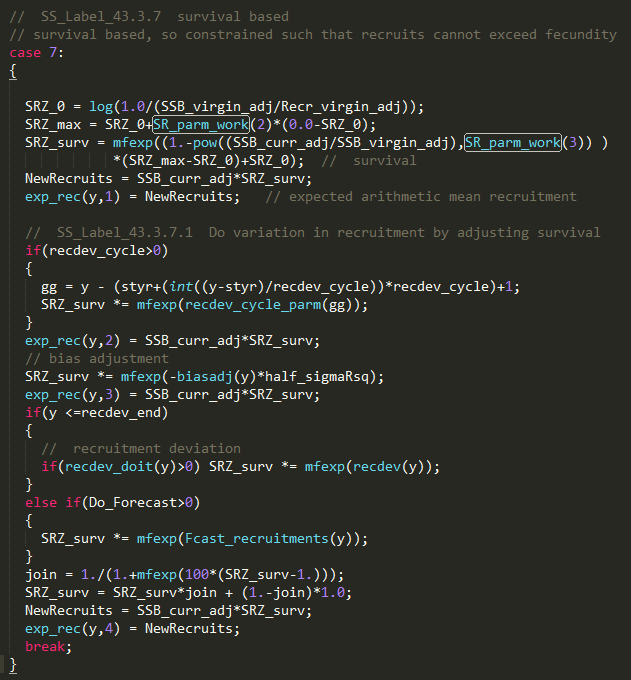
\includegraphics{survival_code_330}

\scriptsize
\begin{verbatim}
//  SS_Label_43.3.7  survival based
case 7:  // survival based, so constrained such that recruits cannot exceed fecundity
{

SRZ_0=log(1.0/(SSB_virgin_adj/Recr_virgin_adj));
SRZ_max=SRZ_0+SR_parm_work(2)*(0.0-SRZ_0);
SRZ_surv=mfexp((1.-pow((SSB_curr_adj/SSB_virgin_adj),SR_parm_work(3)) )*(SRZ_max-SRZ_0)+SRZ_0);  //  survival
NewRecruits=SSB_curr_adj*SRZ_surv;
exp_rec(y,1)=NewRecruits;   // expected arithmetic mean recruitment

//  SS_Label_43.3.7.1  Do variation in recruitment by adjusting survival
if(recdev_cycle>0)
{
gg=y - (styr+(int((y-styr)/recdev_cycle))*recdev_cycle)+1;
SRZ_surv*=mfexp(recdev_cycle_parm(gg));
}
exp_rec(y,2)=SSB_curr_adj*SRZ_surv;
SRZ_surv*=mfexp(-biasadj(y)*half_sigmaRsq);     // bias adjustment
exp_rec(y,3)=SSB_curr_adj*SRZ_surv;
if(y <=recdev_end)
{
if(recdev_doit(y)>0) SRZ_surv*=mfexp(recdev(y));  //  recruitment deviation
}
else if(Do_Forecast>0)
{
SRZ_surv *= mfexp(Fcast_recruitments(y));
}
join=1./(1.+mfexp(100*(SRZ_surv-1.)));
SRZ_surv=SRZ_surv*join + (1.-join)*1.0;
NewRecruits=SSB_curr_adj*SRZ_surv;
exp_rec(y,4) = NewRecruits;
break;
}
\end{verbatim}

\pagebreak
\subsection{Random Walk Selectivity: Pattern 17}
\hypertarget{RandWalkSelex}{Code} for selectivity pattern 17, random walk shown below:
%	\begin{center}
%		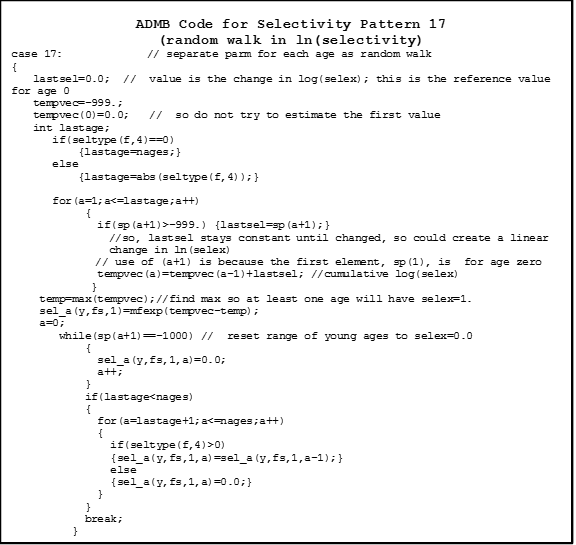
\includegraphics{Selex17_RandomWalk}
%	\end{center}	
\scriptsize{
	\begin{verbatim}
	 
	 //  SS_Label_Info_22.7.17 #age selectivity: each age has parameter as random walk
	 // #41 each age has parameter as random walk scaled by average of values at low age through high age
	 //    transformation as selex=exp(parm); some special codes */
	 case 41:
	 scaling_offset = 2;
	 case 17:                  //
	 {
	 lastsel=0.0;  //  value is the change in log(selex);  this is the reference value for age 0
	 tempvec_a=-999.;
	 tempvec_a(0)=0.0;   //  so do not try to estimate the first value
	 int lastage;
	 if(seltype(f,4)==0)
	 {lastage=nages;}
	 else
	 {lastage=abs(seltype(f,4));}
	 
	 for (a=1;a<=lastage;a++)
	 {
	 //  with use of -999, lastsel stays constant until changed, so could create a linear change in ln(selex)
	 // use of (a+1) is because the first element, sp(1), is for age zero
	 if(sp(a+1+scaling_offset)>-999.) {lastsel=sp(a+1+scaling_offset);}
	 tempvec_a(a)=tempvec_a(a-1)+lastsel;   // cumulative log(selex)
	 }
	 if (scaling_offset == 0)
	 {
	 temp=max(tempvec_a);   //  find max so at least one age will have selex=1.
	 }
	 else
	 {
	 int low_bin  = int(value(sp(1)));
	 int high_bin = int(value(sp(2)));
	 if (low_bin < 0)
	 {
	 low_bin = 0;
	 N_warn++; warning<<" selex pattern 41; value for low bin is less than 0, so set to 0 "<<endl;
	 }
	 if (high_bin > nages)
	 {
	 high_bin = nages;
	 N_warn++; warning<<" selex pattern 41; value for high bin is greater than "<<nages<<", so set to "<<nages<<" "<<endl;
	 }
	 if (high_bin < low_bin) high_bin = low_bin;
	 if (low_bin > high_bin) low_bin = high_bin;
	 sp(1) = low_bin;
	 sp(2) = high_bin;
	 temp=mean(tempvec_a(low_bin,high_bin));
	 }
	 sel_a(y,fs,1)=mfexp(tempvec_a-temp);
	 a=0;
	 while(sp(a+1+scaling_offset)==-1000)  //  reset range of young ages to selex=0.0
	 {
	 sel_a(y,fs,1,a)=0.0;
	 a++;
	 }
	 scaling_offset = 0;     // reset scaling offset
	 if(lastage<nages)
	 {
	 for (a=lastage+1;a<=nages;a++)
	 {
	 if(seltype(f,4)>0)
	 {sel_a(y,fs,1,a)=sel_a(y,fs,1,a-1);}
	 else
	 {sel_a(y,fs,1,a)=0.0;}
	 }
	 }
	 break;
	 }  
	\end{verbatim}

\pagebreak
\subsection{Cubic Spline Selectivity}
\hypertarget{CubicSpline}{Code} for cubic spline selectivity, option 42, shown below:
%	\begin{center}
%		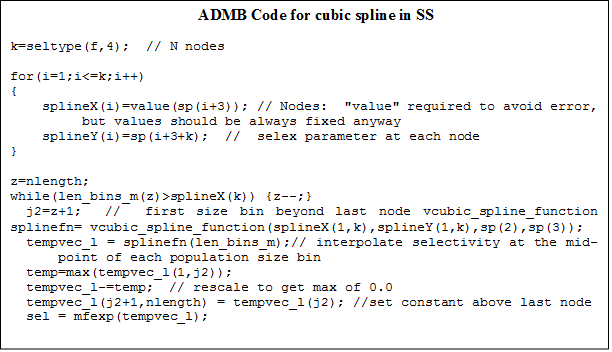
\includegraphics{CubicSplineCode}
%	\end{center}

\scriptsize
\begin{verbatim}
	
	//  SS_Label_Info_22.7.27 #age selectivity: cubic spline
	// #42 cubic spline scaled by average of values at low age through high age
	case 42:
	scaling_offset = 2;
	case 27:
	{
	k=seltype(f,4);  // n points to include in cubic spline
	for (i=1;i<=k;i++)
	{
	splineX(i)=value(sp(i+3+scaling_offset)); // "value" required to avoid error, but values should be always fixed anyway
	splineY(i)=sp(i+3+k+scaling_offset);
	}
	z=nages;
	while(r_ages(z)>splineX(k)) {z--;}
	j2=z+1;  //  first age beyond last node
	vcubic_spline_function splinefn=vcubic_spline_function(splineX(1,k),splineY(1,k),sp(2+scaling_offset),sp(3+scaling_offset));
	tempvec_a= splinefn(r_ages);  // interpolate selectivity at each age
	if (scaling_offset == 0)
	{
	temp=max(tempvec_a(0,j2));
	}
	else
	{
	int low_bin  = int(value(sp(1)));
	int high_bin = int(value(sp(2)));
	if (low_bin < 0)
	{
	low_bin = 0;
	N_warn++; warning<<" selex pattern 42; value for low bin is less than 0, so set to 0 "<<endl;
	}
	if (high_bin > nages)
	{
	high_bin = nages;
	N_warn++; warning<<" selex pattern 42; value for high bin is greater than "<<nages<<", so set to "<<nages<<" "<<endl;
	}
	if (high_bin < low_bin) high_bin = low_bin;
	if (low_bin > high_bin) low_bin = high_bin;
	sp(1) = low_bin;
	sp(2) = high_bin;
	temp=mean(tempvec_a(low_bin,high_bin));
	scaling_offset = 0;     // reset scaling offset
	}
	tempvec_a-=temp;  // rescale to get max of 0.0
	tempvec_a(j2+1,nages) = tempvec_a(j2);  //  set constant above last node
	sel_a(y,fs,1)=mfexp(tempvec_a);
	break;
	}
	
\end{verbatim}

\pagebreak
\subsection{Deviation Link}
\hypertarget{DevLink}{Code} for alternative deviation links shown below:

\scriptsize
\begin{verbatim}

    case 1 (multiplicative):
    {
      for (j=timevary_setup(10);j<=timevary_setup(11);j++)
      {
        parm_timevary(tvary,j)*=mfexp(parm_dev(k,j)*parm_dev_stddev(k));
      }
      break;
    }

    case 2 (additive):
    {
      for (j=timevary_setup(10);j<=timevary_setup(11);j++)
      {
        parm_timevary(tvary,j)+=parm_dev(k,j)*parm_dev_stddev(k);
      }
      break;
    }

    case 3 (random walk):
    {
      parm_dev_rwalk(k,timevary_setup(10))=parm_dev(k,timevary_setup(10))*parm_dev_stddev(k);
      parm_timevary(tvary,timevary_setup(10))+=parm_dev_rwalk(k,timevary_setup(10));
      for (j=timevary_setup(10)+1;j<=timevary_setup(11);j++)
      {
        parm_dev_rwalk(k,j)=parm_dev_rwalk(k,j-1)+parm_dev(k,j)*parm_dev_stddev(k);
        parm_timevary(tvary,j)+=parm_dev_rwalk(k,j);
      }
      break;
    }

    case 4 (mean reverting random walk)
    {
      parm_dev_rwalk(k,timevary_setup(10))=parm_dev(k,timevary_setup(10))*parm_dev_stddev(k);
      parm_timevary(tvary,timevary_setup(10))+=parm_dev_rwalk(k,timevary_setup(10));
      for (j=timevary_setup(10)+1;j<=timevary_setup(11);j++)
      {
        //    =(1-rho)*mean + rho*prevval + dev   //  where mean = 0.0
        parm_dev_rwalk(k,j)=parm_dev_rho(k)*parm_dev_rwalk(k,j-1)+parm_dev(k,j)*parm_dev_stddev(k);
        parm_timevary(tvary,j)+=parm_dev_rwalk(k,j);
      }
      break;
    }
	
\end{verbatim}

\pagebreak